%% Manuscript draft. Compile with pdflatex + bibtex.
%% Numbers kept in sync with results/tables/*.json and *.csv (see manuscript/README.md).
\documentclass[11pt]{article}
\usepackage[margin=1in]{geometry}
\usepackage{amsmath,amssymb,amsthm,mathtools}
\usepackage{graphicx,booktabs,multirow}
\usepackage[colorlinks=true,linkcolor=blue,citecolor=blue]{hyperref}
\hypersetup{pdftitle={Separating Training, Evaluation and Constraint-Set Noise in Fairness Uncertainty Quantification},pdfauthor={Cenfa Lu, Shuda Wu and Xun Liu},
  pdfkeywords={fairness auditing, uncertainty quantification, constrained stochastic optimization, online bootstrap, distribution-free inference},
  pdfsubject={Fairness uncertainty quantification: training, evaluation and constraint-set noise}}
\usepackage{natbib}
\bibliographystyle{plainnat}

\newtheorem{theorem}{Theorem}
\newtheorem{lemma}{Lemma}
\newtheorem{corollary}{Corollary}
\newtheorem{proposition}{Proposition}
\newtheorem{assumption}{Assumption}
\newtheorem{remark}{Remark}

\newcommand{\E}{\mathbb{E}}
\newcommand{\R}{\mathbb{R}}
\newcommand{\phidi}{\phi_{\mathrm{DI}}}
\newcommand{\phidm}{\phi_{\mathrm{DM}}}
\newcommand{\dhat}{\hat\Delta}
\newcommand{\tbar}{\bar\theta}
\newcommand{\Dp}{D'}
\newcommand{\Dt}{\tilde D}

\title{Separating Training, Evaluation and Constraint-Set Noise\\in Fairness Uncertainty Quantification}
% ==AUTHOR-BLOCK-START==
\author{Cenfa Lu\thanks{\href{https://orcid.org/0009-0003-3481-3624}{ORCID: 0009-0003-3481-3624}; \texttt{joffin@163.com}}\\
Shuda Wu\thanks{\href{https://orcid.org/0009-0003-2590-9608}{ORCID: 0009-0003-2590-9608}; \texttt{shudawu777@163.com}}\\
Xun Liu\thanks{\href{https://orcid.org/0009-0005-4230-3047}{ORCID: 0009-0005-4230-3047}; \texttt{liuxun0817@163.com}}\\
School of Mathematics and Computing Science,\\
Guilin University of Electronic Technology, Guilin 541004, China\\
\textit{Corresponding author: Cenfa Lu (\texttt{joffin@163.com})}}
% ==AUTHOR-BLOCK-END==
\date{}

\begin{document}
\maketitle

\begin{abstract}
Fairness-aware classifiers trained by stochastic gradient methods are themselves random, and so is any
demographic-parity or equalised-odds gap computed from them.  Recent work builds confidence intervals
for such gaps with an online multiplier bootstrap, but those intervals track only the random variation
of the optimisation trajectory.  With a finite held-out set, a second component, the sampling noise of
the evaluation sample, is ignored, often the larger of the two; a third source enters when
the constraint set that defines the target is itself drawn at random.  We decompose this error into training and evaluation parts, derive the limiting distribution of the sum, and give the closed-form asymptotic coverage of the existing interval as a function of the ratio of
training iterations to evaluation size; the interval is valid only when the evaluation set is large
relative to the training run.  We then propose a joint bootstrap that resamples both the training
trajectories and the evaluation set, adding a constraint-set layer when the audit design is random,
prove its asymptotic validity for a fixed design, and give a sample-size allocation rule.  In a
reproduction on synthetic data, Adult, ACSIncome and COMPAS, the existing interval covers the population fairness gap in $0$--$62\%$ of repetitions on the three real audits, whereas the joint interval is close to nominal on Adult ($0.98$ versus $0.30$).  A variance budget attributes only $0.8\%$--$8.3\%$ of the variability to training noise.

\par\medskip\noindent\textbf{Keywords:} fairness auditing; uncertainty quantification; constrained stochastic optimization; online bootstrap; distribution-free inference.
\end{abstract}

\section{Introduction}
\label{sec:intro}

Machine-learning models used in high-stakes decisions are increasingly required to report fairness
diagnostics such as the demographic-parity (DP) gap or the equalised-odds (EO) gap between protected
groups \citep{hardt2016,corbett2017}.  In practice these diagnostics are computed from a finite
held-out sample for a classifier whose parameters were themselves produced by a stochastic
optimisation algorithm.  Both steps inject randomness, and a point estimate without an accompanying uncertainty statement is
of limited use for an audit.

\citet{roy2026uq} take up this problem for fairness-aware linear classifiers trained online by
stochastic dual averaging (for DP) or penalised SGD (for EO-type criteria).  Viewing training as
constrained stochastic optimisation, they establish asymptotic normality of the averaged iterate, and
because the asymptotic covariance depends on the unknown optimum they propose an online multiplier
bootstrap operating on a single data stream.  Computing the interval is cheap: the trajectories can be run in parallel and no retraining is
required.

Our starting point is the estimand such an interval actually covers.  Write
$\theta^*$ for the population optimum of the fairness-aware objective, $\tbar_T$ for the averaged
online iterate after $T$ steps, and $\dhat_m$ for the empirical fairness gap computed on an
independent held-out set $\Dt$ of size $m$.  The reported number is $\dhat_m(\tbar_T)$, while the
quantity a deployment decision depends on is the population gap $\Delta(\theta^*)$.  The error
splits into
\[
\dhat_m(\tbar_T)-\Delta(\theta^*)
=\underbrace{\Delta(\tbar_T)-\Delta(\theta^*)}_{\text{training}}
+\underbrace{\dhat_m(\tbar_T)-\Delta(\tbar_T)}_{\text{evaluation}} ,
\]
and the two terms are independent because $\Dt$ is independent of the training stream.
The online bootstrap approximates the law of the first term only.  If the evaluation error is small relative to the training noise, the distinction can be ignored; in the regimes we study it cannot be.  In our reproduction with $m=1000$ held-out observations the evaluation standard error for Adult is
$4.6$ times the training standard error (Table~\ref{tab:budget}); the existing interval covers the
population gap in $30\%$ of repetitions, not the nominal $95\%$.

\paragraph{Contributions.}
\begin{enumerate}
  \item \emph{Decomposition and a diagnostic.}  We show that the error of the reported gap relative to
        a fixed audit design decomposes into two asymptotically independent components, training and
        evaluation sampling, and into a third, design component that arises when the constraint set is
        itself a random draw.  We derive the limiting distribution (Theorem~\ref{thm:limit}) and the
        closed-form asymptotic coverage of the existing interval (Corollary~\ref{cor:coverage}).  The
        interval is asymptotically valid only when $m \gg T\,v^2/\sigma^2_\Delta$, a condition that the published setups violate by factors of $4.5$ to $79$ (Table~\ref{tab:budget}).
  \item \emph{A joint bootstrap.}  We combine the multiplier bootstrap over training trajectories with
        resampling of the evaluation set, and add an outer bootstrap over the constraint set when the
        design is random.  The two-source construction is asymptotically valid for a fixed audit design
        (Theorem~\ref{thm:joint}).  It costs a few vectorised passes over the held-out predictions, and the
        design layer adds a small number of direct constrained solves.
  \item \emph{A variance budget and design guidance.}  On Adult, ACSIncome and COMPAS the training
        component accounts for only $0.8$--$8.3\%$ of the variability of a reported gap; the
        dominant components are evaluation sampling ($37$--$78\%$) and constraint-set sampling
        ($18$--$55\%$).  This yields a rule for allocating audit effort between training
        iterations, labelled evaluation data and the choice of constraint set.
  \item \emph{A reproducible study.}  We re-implement the baseline from the published equations
        (no official code was released), reproduce its qualitative claims on five data settings, and
        document two further reproducibility findings: the published step-size schedule does not reach the reported convergence regime, and the synthetic data generator is close to
        degenerate.  All code, data splits and raw results are released.
\end{enumerate}

Section~\ref{sec:related} reviews related work.  Sections~\ref{sec:setup} and~\ref{sec:decomp} fix notation and state the decomposition, Section~\ref{sec:method} describes the joint bootstrap, and Section~\ref{sec:exp} reports the experiments.  Section~\ref{sec:discussion} discusses limitations and practical consequences.

\section{Related work}
\label{sec:related}

\paragraph{Online inference for stochastic approximation.}
Asymptotic normality of averaged stochastic approximation goes back to
\citet{polyak1992}; constrained variants are analysed by \citet{duchi2016}.  Online bootstrap and
online covariance procedures for unconstrained SGD are developed by \citet{fang2018,chen2016,zhu2021} and
extended to policy evaluation \citep{ramprasad2023}.  These methods target the model parameter, whereas a fairness gap is a non-smooth functional of it;
\citet{roy2026uq} derive the limiting distribution of that functional under constrained stochastic
approximation and estimate it with an online multiplier bootstrap.  We leave
the training-side theory in place and add the evaluation component; the constraint-set (design)
component is treated separately, as variability of the target rather than of the estimate.

\paragraph{Statistical inference for fairness.}
A parallel literature tests whether a \emph{fixed} classifier is fair: permutation tests
\citep{diciccio2020}, optimal-transport projections \citep{taskesen2021}, adversarial individual-fairness
tests \citep{maity2021}, and bootstrap audits over rich group collections \citep{cherian2023}.  These
papers treat the classifier as given and quantify evaluation uncertainty only, which is the
complementary half of our decomposition.  Our method targets the composition of training and
evaluation uncertainty and makes the two components separately reportable.

\paragraph{Uncertainty in fairness more broadly.}
\citet{rosenblatt2024} benchmark uncertainty estimates in fair predictive pipelines, a different
object from sampling uncertainty about the fairness of a trained predictor.  Subgroup-level fairness estimates also carry
estimation variance that grows as the subgroup shrinks (Lemma~\ref{lem:eval}); our evaluation
component formalises this in the DI/DM setting and is combined with the training component rather
than studied in isolation.

\paragraph{Reproducibility and its use here.} Neither the UAI proceedings version nor the earlier arXiv version \citep{roy2023uq} ships official code, so we
re-implemented both training procedures and the multiplier bootstrap from the published equations and
report a full reproduction study.  The qualitative claims reproduce: the mean interval score
decreases with the number of iterations, the empirical distribution of the estimated gap converges to
the benchmark normal law in Wasserstein-2 distance, and the interval covers the held-out estimand.
Two discrepancies are documented.  The published step-size schedule ($\eta_k=0.01k^{-0.501}$) does not reach the convergence regime shown in the paper within $10^6$ iterations.  The synthetic generator
is also close to degenerate, since the protected attribute is highly correlated with the label
(correlation $0.83$).  We
therefore calibrate the step size (and, on real data, the regularisation strength) and report both
the paper-literal and the calibrated settings.

\section{Problem setup}
\label{sec:setup}

\paragraph{Data and classifier.} Let $(x,y,z)\sim P$ with features $x\in\R^p$, label
$y\in\{-1,1\}$ and protected attribute $z\in\{0,1\}$.  We consider linear classifiers
$h(x;\theta)=\operatorname{sign}(\theta^\top\varphi(x))$ with $\varphi(x)=(x^\top,1)^\top
\in\R^d$, $d=p+1$.

\paragraph{Disparate impact.} With tolerance $\epsilon>0$ and a held-out constraint set
$\Dp$ of size $n_c$, define
$\tilde x=n_c^{-1}\sum_{i\in\Dp}(z_i-\bar z)\varphi(x_i)$ and
$\Theta(\Dp)=\{\theta:|\tilde x^\top\theta|\le\epsilon\}$.  The target parameter is
\begin{equation}\label{eq:theta}
\theta^*=\arg\min_{\theta\in\Theta(\Dp)}\ \ell(\theta),\qquad
\ell(\theta)=\E[\log(1+e^{-y\theta^\top\varphi(x)})]+\frac{\kappa}{2}\|\theta\|_2^2 ,
\end{equation}
and the population gap is $\Delta(\theta)=P(h=1\mid z=0)-P(h=1\mid z=1)$ with
$\phi(\theta)=|\Delta(\theta)|$.

\paragraph{Disparate mistreatment.} With penalty $R^2>0$ and $\Dp_-=\{i\in\Dp:y_i=-1\}$,
$\gamma(\theta;\Dp_-)=\big(n_-^{-1}\sum_{i\in\Dp_-}(z_i-\bar z)\min(0,y_i\varphi(x_i)^\top
\theta)\big)^2$ and $\theta^*=\arg\min_\theta \ell(\theta)+R^2\gamma(\theta;\Dp_-)$; the population
gap conditions on $y=-1$.

\paragraph{Online training.} The averaged iterate $\tbar_T=T^{-1}\sum_{k=1}^T\theta_k$ is produced by
stochastic dual averaging with projection onto $\Theta(\Dp)$ for DP, or by penalised SGD for EO.  An
online multiplier bootstrap with $B$ perturbed trajectories, each driven by the same single data
stream with i.i.d.\ multipliers $V\sim\mathrm{Unif}[1-\sqrt3,1+\sqrt3]$, yields
$\{\hat\theta^b_T\}_{b=1}^B$ and hence $\{\dhat_m(\bar\theta^b_T)\}$; see \citet{roy2026uq} for the
algorithm and its training-side guarantees.

\paragraph{Two estimands.} Notation is collected in Table~\ref{tab:notation}.  We distinguish the \emph{held-out estimand} $\dhat_m(\theta^*)$, i.e.\ the
fairness of the optimal classifier evaluated on the very sample used by the auditor, from the
\emph{population estimand} $\Delta(\theta^*)$, i.e.\ the fairness of the deployed classifier on the
data distribution.  The distinction disappears only as $m\to\infty$, so a confidence interval must name its target.

\begin{table}[t]
\centering
\small
\caption{Notation.}
\label{tab:notation}
\begin{tabular}{ll}
\toprule
symbol & meaning \\
\midrule
$\theta$ & linear-classifier parameter; $h(x;\theta)=\operatorname{sign}(\theta^\top\varphi(x))$ \\
$\theta^*$ & population constrained optimum \eqref{eq:theta} \\
$\tbar_T$ & averaged online iterate after $T$ steps \\
$\Dp$, $n_c$ & constraint set (audit design) and its size \\
$\Dt$, $m$ & held-out evaluation set and its size \\
$\Delta(\theta)$, $\dhat_m(\theta)$ & population and empirical fairness gap \\
$\sigma^2_\Delta$, $v^2$ & training and evaluation variance constants \\
$\lambda=T/m$ & training-to-evaluation effort ratio \\
$\sigma^2_{\rm tot}$ & $\sigma^2_\Delta+\lambda v^2$, limiting variance of the reported gap \\
$B$ & number of multiplier-bootstrap trajectories \\
$Q$ & number of evaluation resamples \\
$\eta_k$, $\kappa$, $R$ & step size, $L_2$ regularisation, mistreatment penalty \\
\bottomrule
\end{tabular}
\end{table}

\section{Decomposition: two error sources and a design component}
\label{sec:decomp}

\begin{assumption}[adapted from \citealp{roy2026uq}]
\label{ass:base}
The loss is strongly convex and smooth on a neighbourhood of $\theta^*$; the data stream is i.i.d.;
the decision boundary is linear in $\theta$; the conditional feature distributions admit continuous
densities at the boundary.  The evaluation set $\Dt$ is drawn i.i.d.\ from $P$ independently of the
training stream and of $\Dp$.
\end{assumption}

All statements in this section condition on the realised constraint set $\Dp$.  Randomness in $\Dp$
enters through the target $\theta^*$ rather than through the estimator, and is analysed separately
in the variance budget of Section~\ref{sec:exp}.

\begin{lemma}[training noise; \citealp{roy2026uq}]
\label{lem:train}
Under Assumption~\ref{ass:base},
$\sqrt T(\Delta(\tbar_T)-\Delta(\theta^*))\Rightarrow\mathcal N(0,\sigma^2_\Delta)$ with
$\sigma^2_\Delta=g^\top\Sigma g$, $g=\nabla\Delta(\theta^*)$, and $\Sigma$ the asymptotic covariance
of the averaged iterate.
\end{lemma}

\begin{lemma}[evaluation noise]
\label{lem:eval}
Under Assumption~\ref{ass:base}, uniformly over $\theta$ in a neighbourhood of $\theta^*$,
\[
\sqrt m\big(\dhat_m(\theta)-\Delta(\theta)\big)\Rightarrow\mathcal N\!\big(0,\,v^2(\theta)\big),
\qquad
v^2(\theta)=\frac{p_0(1-p_0)}{P(z=0)}+\frac{p_1(1-p_1)}{P(z=1)},
\]
with $p_j=P(h=1\mid z=j)$, and the analogous expression with $y=-1$ for DM.  Moreover the two
convergences are independent.
\end{lemma}

\begin{theorem}[limit distribution]
\label{thm:limit}
Suppose $\Delta(\theta^*)\neq0$ and $T,m\to\infty$ with $T/m\to\lambda\in[0,\infty)$.  Then under
Assumption~\ref{ass:base},
\[
\sqrt T\big(\dhat_m(\tbar_T)-\Delta(\theta^*)\big)\Rightarrow
\mathcal N\big(0,\ \sigma^2_\Delta+\lambda v^2\big),
\qquad\text{conditionally on }\Dp.
\]
\end{theorem}

\begin{corollary}[coverage of the existing interval]
\label{cor:coverage}
The fixed-time interval of \citet{roy2026uq}, of asymptotic half-width
$z_{\alpha/2}\sigma_\Delta/\sqrt T$, has asymptotic coverage
\[
2\Phi\!\Big(z_{\alpha/2}\,\frac{\sigma_\Delta}{\sqrt{\sigma^2_\Delta+\lambda v^2}}\Big)-1,
\]
which equals $1-\alpha$ if and only if $\lambda v^2/\sigma_\Delta^2\to0$, i.e.\
$m\gg T v^2/\sigma_\Delta^2$.
\end{corollary}

\begin{remark}[two coverage protocols]
\label{rem:protocol}
If the evaluation set $\Dt$ is held fixed across repetitions, as in the original simulation design,
the evaluation error becomes a constant bias $b=\dhat_m(\theta^*)-\Delta(\theta^*)$ and coverage is
$\Phi(z_{\alpha/2}-|b|\sqrt T/\sigma_\Delta)-\Phi(-z_{\alpha/2}-|b|\sqrt T/\sigma_\Delta)$.
Coverage statements about population fairness must therefore be evaluated with a fresh evaluation
set in each repetition; we report both protocols.
\end{remark}

\section{Method: joint bootstrap}
\label{sec:method}

For $b=1,\dots,B$ multiplier trajectories, $r=1,\dots,Q$ evaluation resamples, and $s=1,\dots,S$ constraint-set resamples, define the bootstrap deviations
\[
D^*_{b,r,s}
= \underbrace{\dhat_m(\bar\theta^b_T)-\dhat_m(\tbar_T)}_{\text{training}}
+ \underbrace{\dhat_{m,r}(\tbar_T)-\dhat_m(\tbar_T)}_{\text{evaluation}}
+ \underbrace{\dhat_{m}(\theta^*_s)-\dhat_m(\theta^*)}_{\text{constraint set}} ,
\]
where the third term uses the constrained optimum $\theta^*_s$ computed for a resampled constraint
set $\Dp_s$; it is obtained by solving the constrained problem directly, with no retraining.
The proposed interval is
$\big[\dhat_m(\tbar_T)+\hat q_{\alpha/2},\ \dhat_m(\tbar_T)+\hat q_{1-\alpha/2}\big]$
for the quantiles of $D^*$, mapped to $|\Delta|$ by folding: if the resulting interval for the signed
gap excludes zero we report the absolute values of its endpoints, otherwise we report
$[0,\max(|l|,|u|)]$.  When the constraint set is fixed by design the third term is omitted, and the interval targets
$\Delta(\theta^*)$ for the realised $\Dp$.  All experiments below use this fixed-design version, so
the coverage reported there concerns the two inference-error components; the design layer is
quantified separately in the variance budget.

\begin{theorem}[asymptotic validity]
\label{thm:joint}
Under Assumption~\ref{ass:base}, if $\tbar_T\to\theta^*$ and the constraint set is fixed by
design (third term omitted), then conditionally on the data the law of $D^*$ converges in
probability to the law of $\dhat_m(\tbar_T)-\Delta(\theta^*)$; consequently the percentile interval
has asymptotic coverage $1-\alpha$ for $\phi(\theta^*)$.  If the design is random and the third term is included, the conclusion holds for the design-conditional target as $S\to\infty$, and the interval is conservative for a realised design because the added term has mean zero and is asymptotically independent of the first two.
\end{theorem}

\paragraph{Cost.} The evaluation resampling is a vectorised operation on the $m$ held-out
predictions and costs $O(Qm)$.  The training deviation reuses the $B$ trajectories already produced
by the online bootstrap.  The constraint-set bootstrap requires $S$ direct constrained solves, each
costing a few iterations of a standard constrained solver, and no additional passes over the data
stream.

\paragraph{Sample-size allocation.}
\label{sec:ss}
With per-unit costs $c_T$ and $c_m$ and target half-width $w$, minimising $c_T T+c_m m$ subject to
$z_{\alpha/2}^2(\sigma^2_\Delta/T+v^2/m)\le w^2$ gives
\[
\frac{m}{T}=\sqrt{\frac{v^2c_T}{\sigma^2_\Delta c_m}},\qquad
T=\frac{z_{\alpha/2}^2}{w^2}\Big(\sigma^2_\Delta+\sigma_\Delta v\sqrt{c_m/c_T}\Big).
\]
Because the evaluation variance is not negligible in the regimes we study, the binding
constraint is the \emph{absolute} size of $m$: increasing $T$ alone cannot push the half-width below
$z_{\alpha/2}v/\sqrt m$ (Figure~\ref{fig:samplesize}).

\section{Experiments}
\label{sec:exp}

\paragraph{Setup and protocols.} Synthetic data follow the generators of \citet{zafar2019} used by
\citet{roy2026uq}; real data are Adult and ACSIncome \citep{ding2021} and COMPAS, with the sensitive attributes and tolerances of Table~1 in the original paper.  Three protocols appear below.
\emph{(R) Reproduction}: one fixed constraint set and one fixed held-out set, repetitions resample
only the training stream, which is the protocol of the original simulation study.
\emph{(A) Protocol A}: the constraint set is fixed but every repetition draws a fresh evaluation set
from a disjoint reservoir, so that coverage is evaluated over the evaluation sampling law as well.
\emph{(B) Budget}: the audit budget reported in practice ($T=3\times10^4$, $m=1000$ for
Adult/ACSIncome and $m=400$ for COMPAS), which is the operating point marked in
Figure~\ref{fig:samplesize}; the planning analysis uses the component estimates of protocol (A) at
this budget.  Unless stated otherwise $B=100$ multiplier trajectories, $Q=300$ evaluation resamples and $\alpha=0.05$; step size and regularisation are calibrated as
described above ($\eta_0=0.1$ for DI, $0.03$ for the synthetic DM generator, $\kappa=0.1$).  The
constraint set is held fixed at the sampled audit design in all three protocols, so the joint
interval used below is the two-source version; the constraint-set layer is quantified separately
in the variance budget.

\paragraph{Reproduction of the baseline.}
Table~\ref{tab:repro} summarises the reproduced behaviour in the original fixed-held-out protocol.  The
qualitative claims of the baseline hold: the mean interval score decreases with $T$, the empirical distribution converges to the benchmark normal law, and the interval covers the held-out estimand in $0.86$--$1.00$ of repetitions.  For the population estimand, coverage ranges from $0.00$ to $0.62$ except in the synthetic DM setting,
where the interval width ($0.208$) exceeds the evaluation bias ($0.057$) and the population target is
covered as well.

Figures~\ref{fig:reprodi} and~\ref{fig:reprocompas} show the per-iteration
trajectories behind these numbers.  Convergence to the asymptotic law is fast on the synthetic experiment.  The population estimand is missed as soon as the evaluation error is comparable to the interval width.  A separate grid of training horizons makes the $T^{-1/2}$ rate behind Theorem~\ref{thm:limit} visible: the distance of $\tbar_T$ to the constrained optimum decays with log--log slope $0.47$, and the signed training bias of the gap decays with slope $0.46$ (empirical convergence rates in the supplementary material).

\begin{figure}[t]
\centering
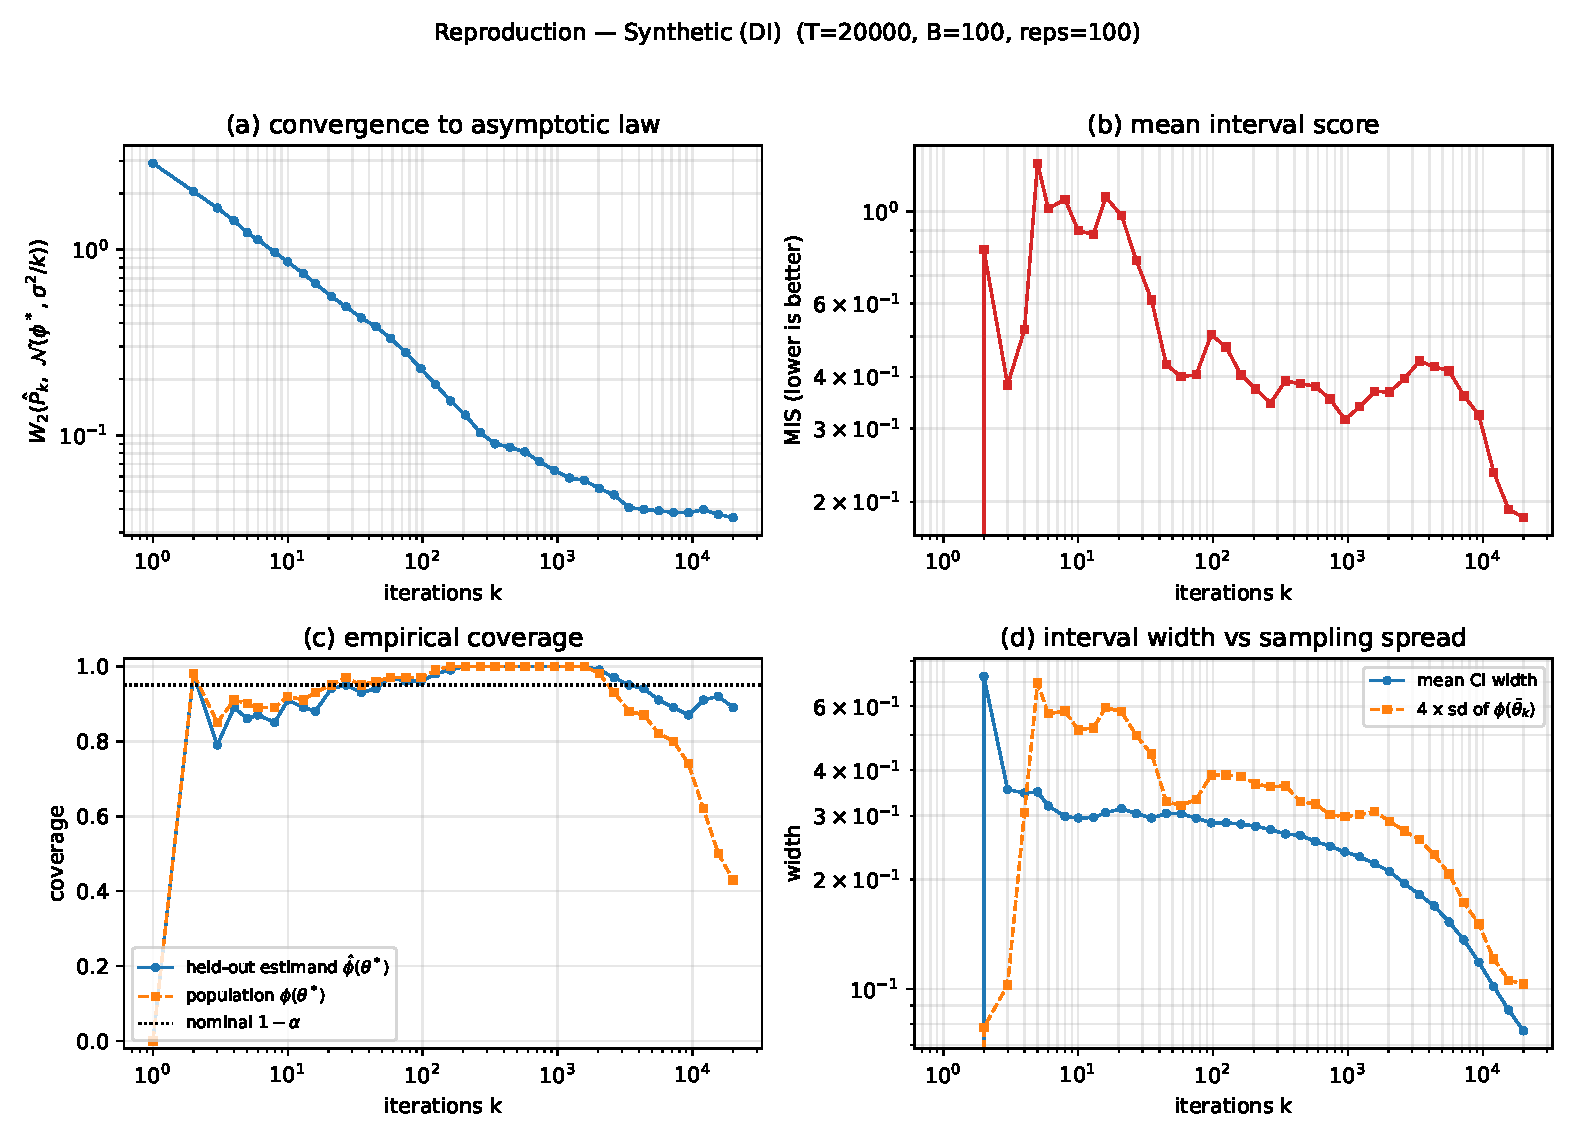
\includegraphics[width=\textwidth]{../results/figures/repro_synth_di.pdf}
\caption{The existing interval tracks the training noise but not the evaluation target.
Reproduction of the synthetic DI experiment: (a) Wasserstein distance between the empirical
law of $\dhat_m(\tbar_T)$ and its asymptotic limit; (b) mean interval score; (c) coverage of the
held-out estimand $\dhat_m(\theta^*)$ and of the population estimand $\Delta(\theta^*)$;
(d) interval width against the sampling spread $4v/\sqrt m$.  The interval covers the held-out
estimand in most repetitions ($0.89$) but the population estimand in only $0.43$.}
\label{fig:reprodi}
\end{figure}

\begin{figure}[t]
\centering
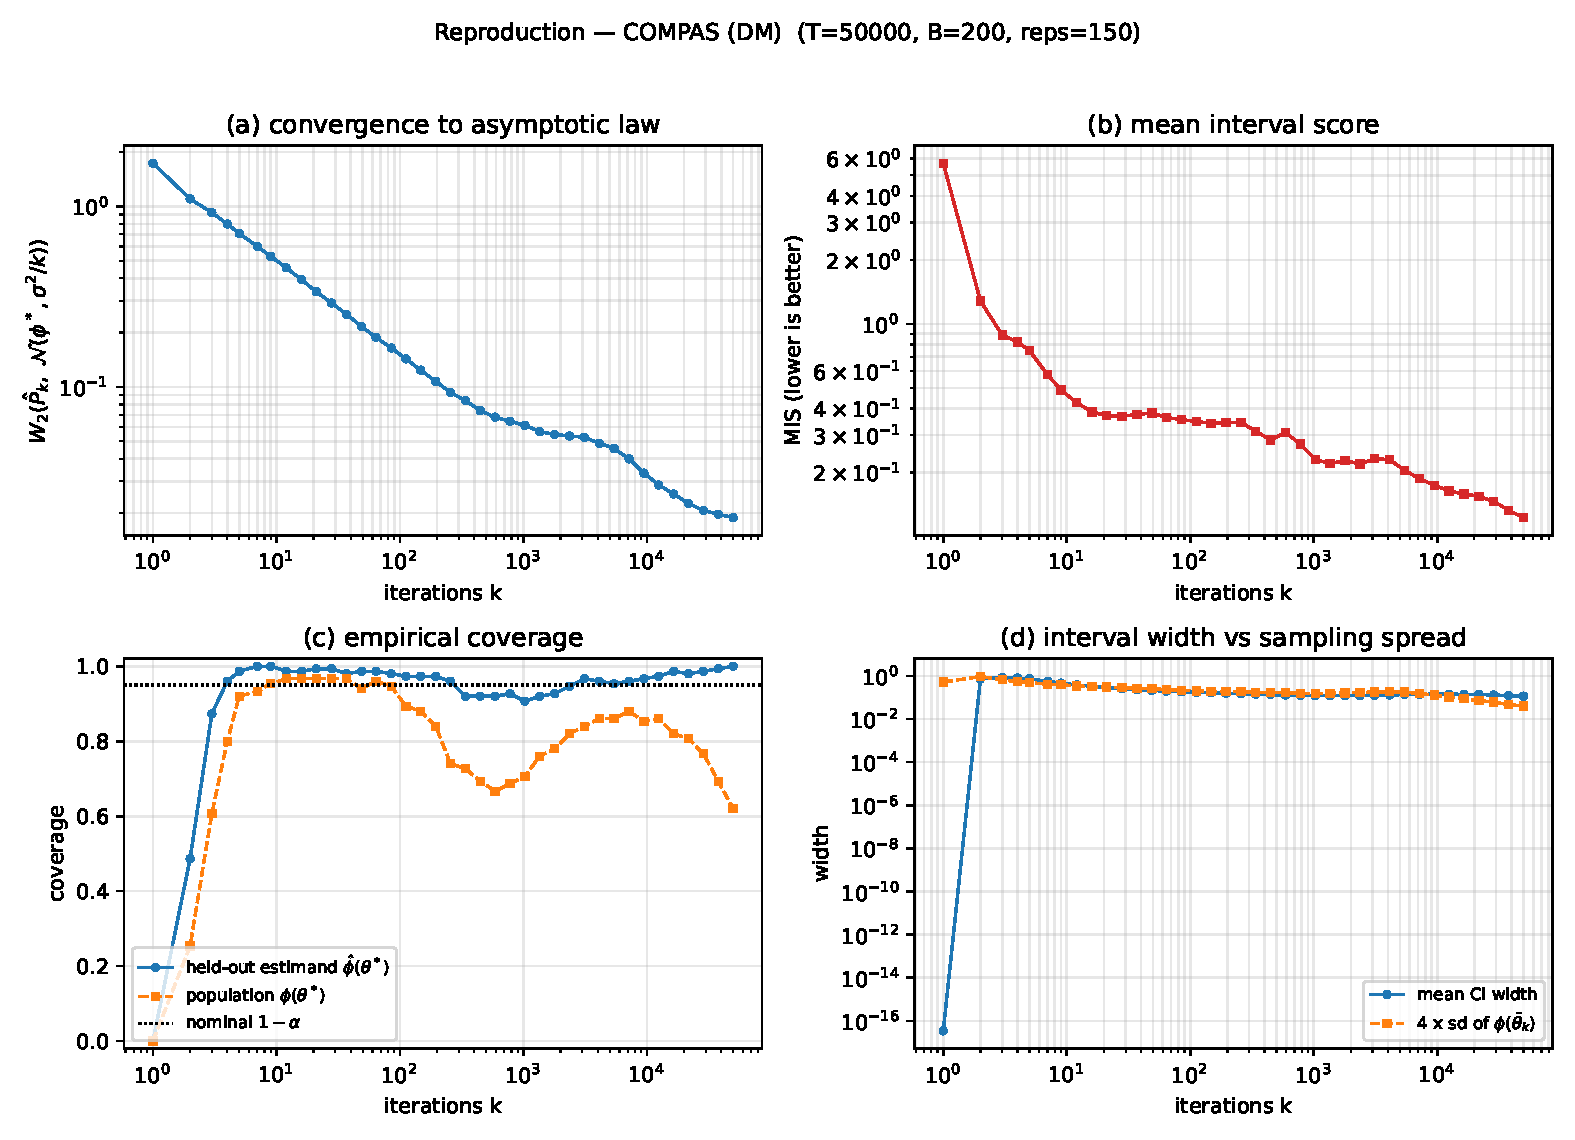
\includegraphics[width=\textwidth]{../results/figures/repro_compas.pdf}
\caption{Evaluation sampling error alone can erase coverage.  Same four panels for the COMPAS DM
experiment.  The interval is centred on the held-out estimand, which it covers in every repetition;
the population estimand differs from it by the sampling error of the evaluation sample, which is
comparable to the interval half-width ($0.062$ against $0.058$), so the population target is covered
in only $0.62$ of repetitions.}
\label{fig:reprocompas}
\end{figure}

\begin{table}[t]
\centering
\small
\setlength{\tabcolsep}{4pt}
\caption{Reproduction of the baseline in the fixed-held-out protocol.  ``coverage held-out'' is the
fraction of repetitions whose interval contains $\dhat_m(\theta^*)$; ``coverage population'' uses
$\Delta(\theta^*)$ evaluated on the full data.}
\label{tab:repro}
\begin{tabular}{lcccccc}
\toprule
setting & $T$ & reps & $\phi(\theta^*)$ & cov.\ held-out & cov.\ population & width \\
\midrule
Synthetic (DI) & 2e4 & 100 & 0.0835 & 0.89 & 0.43 & 0.077 \\
Synthetic (DM) & 2e4 & 100 & 0.1401 & 0.86 & 1.00 & 0.208 \\
Adult (DI)     & 5e4 & 100 & 0.0564 & 1.00 & 0.00 & 0.022 \\
ACSIncome (DI) & 5e4 & 150 & 0.0442 & 1.00 & 0.00 & 0.013 \\
COMPAS (DM)    & 5e4 & 150 & 0.0133 & 1.00 & 0.62 & 0.115 \\
\bottomrule
\end{tabular}
\end{table}

\paragraph{Protocol-A coverage.}
Table~\ref{tab:protocolA} varies the held-out size $m$ with a fresh evaluation set per repetition.
Baseline coverage increases with $m$ as Corollary~\ref{cor:coverage} predicts, while the joint
bootstrap stays at or above nominal coverage.  Its width approaches that of the baseline as $m$ grows,
so the width cost of valid inference is explicit.  The same pattern holds on the three real
datasets, where the baseline interval attains $0.25$--$0.62$ coverage and the joint interval
$0.98$--$1.00$.

\begin{table}[t]
\centering
\small
\setlength{\tabcolsep}{4pt}
\caption{Protocol-A coverage of the population gap (nominal $0.95$) with a fresh evaluation set in
every repetition and a fixed constraint set (two-source joint interval).  Synthetic DI: $T=2\times10^4$, $B=100$, $Q=400$, 100 repetitions, $\phi(\theta^*)=0.0212$ on the population, which is why the target differs from the fixed-held-out one in Table~\ref{tab:repro}.  Real data: $T=3\times10^4$, $B=100$, $Q=300$, 60 repetitions.}
\label{tab:protocolA}
\begin{tabular}{lcccccc}
\toprule
setting & $m$ & cov.\ base & cov.\ joint & $w$ base & $w$ joint & ratio \\
\midrule
Synthetic (DI) & 100  & 0.56 & 0.99 & 0.107 & 0.283 & 2.64 \\
Synthetic (DI) & 1000 & 0.85 & 0.98 & 0.077 & 0.116 & 1.50 \\
Synthetic (DI) & 5000 & 0.99 & 1.00 & 0.074 & 0.085 & 1.15 \\
Adult (DI)     & 1000 & 0.30 & 0.98 & 0.025 & 0.102 & 4.15 \\
ACSIncome (DI) & 1000 & 0.25 & 1.00 & 0.015 & 0.082 & 5.72 \\
COMPAS (DM)    & 400  & 0.62 & 1.00 & 0.096 & 0.173 & 2.08 \\
\bottomrule
\end{tabular}
\end{table}

\paragraph{Variance budget.}
Table~\ref{tab:budget} separates the three sources of variability in a reported gap.  The training
and evaluation components are errors of the reported number around a fixed target; the
constraint-set component measures how far the target itself moves when the audit design is redrawn,
and is therefore a design sensitivity rather than an inferential uncertainty.  Training noise, the only component the baseline addresses, contributes between $0.8\%$ and $8.3\%$ of
the total.  The design component is largest for COMPAS, where its standard error ($0.0753$) is several times the reported gap ($0.0133$), so resampling $\Dp$ can change the sign of the reported gap; a single constrained run is therefore not a reliable audit without a design-sensitivity statement.

\begin{table}[t]
\centering
\small
\setlength{\tabcolsep}{4pt}
\caption{Variance budget: standard errors of the two error components (training, evaluation) and of
the constraint-set (design) component that shifts the target, with shares of the total variability;
the design column is a sensitivity of the audit, not an inferential uncertainty.}
\label{tab:budget}
\begin{tabular}{lcccccc}
\toprule
dataset & se(train) & se(eval) & se($\Dp$) & share(train) & share(eval) & share($\Dp$) \\
\midrule
Adult (DI)     & 0.0056 & 0.0259 & 0.0124 & 3.6\% & 78.3\% & 18.1\% \\
ACSIncome (DI) & 0.0034 & 0.0304 & 0.0245 & 0.8\% & 60.3\% & 39.0\% \\
COMPAS (DM)    & 0.0293 & 0.0621 & 0.0753 & 8.3\% & 37.1\% & 54.6\% \\
\bottomrule
\end{tabular}
\end{table}

\paragraph{Sample-size planning and the minimum certifiable gap.}
Table~\ref{tab:budget} and the planning formula of Section~\ref{sec:ss} together answer a practical
question: at a given audit budget, which fairness gaps can be certified at all?  With the component
estimates from the protocol-A runs, the best achievable $95\%$ half-width at $T=3\times10^4$ and
$m=1000$ is $0.053$ for Adult, $0.060$ for ACSIncome and $0.133$ for COMPAS ($m=400$).  The reported
population gaps are $0.059$, $0.041$ and $0.006$, so at these budgets a zero gap can be excluded for
Adult only; for ACSIncome and COMPAS the minimum certifiable gap exceeds the gap itself, by factors of
$1.5$ and $21$.  Figure~\ref{fig:samplesize} shows the feasible $(T,m)$ region for several target
half-widths.  Since the evaluation variance is not negligible, more training alone does not reduce the
width below the floor $z_{\alpha/2}v/\sqrt m$; only more evaluation data can.

\begin{figure}[t]
\centering
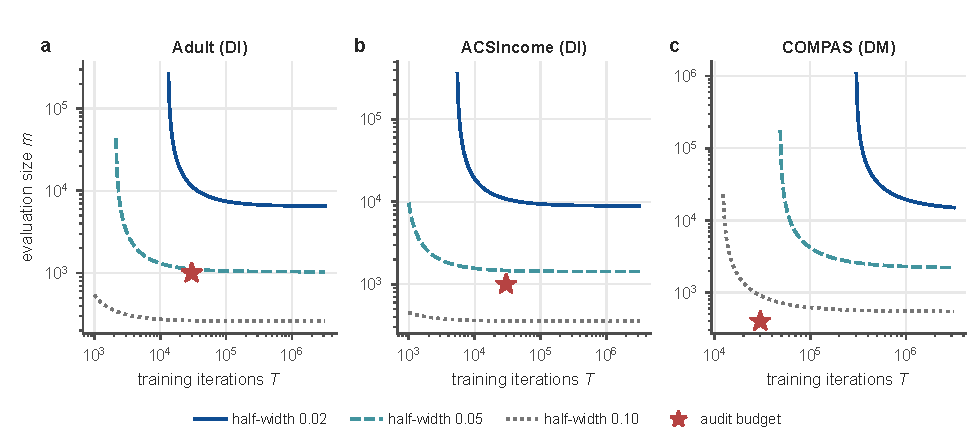
\includegraphics[width=\textwidth]{../results/figures/sample_size.pdf}
\caption{More evaluation data, not more training, buys a narrower interval.  Feasible $(T,m)$
region for target $95\%$ half-widths (curves); the star marks the audit budget ($T=3\times10^4$,
with $m=1000$ for Adult and ACSIncome and $m=400$ for COMPAS).  Points below the curve for a target half-width cannot certify that half-width.}
\label{fig:samplesize}
\end{figure}

\paragraph{Optimisation bias.}
\label{par:bias}
A variance-based interval presumes that the averaged iterate has reached the neighbourhood of
$\theta^*$.  Table~\ref{tab:sensitivity} varies the regularisation strength on Adult under protocol
(R).  At $\kappa=10^{-4}$ the optimum has norm $10.9$ and the averaged iterate is $10.5$ away from
it: no interval based on the training variance can be valid.  The table also shows that coverage is
governed by the \emph{functional} bias of $\phi$, not by the parameter distance: at $\kappa=10^{-2}$
the parameter bias is $0.81$ yet coverage is nominal, while at $\kappa=0.1$ a parameter bias of
$0.12$ is enough to lose all coverage because the DI functional shifts by more than the half-width
(DP/DM gaps are discontinuous in $\theta$).  Audits should therefore report a convergence diagnostic
together with the interval, and the optimisation bias must be controlled by the design ($T$ and
$\kappa$), not by the bootstrap.

\begin{table}[t]
\centering
\caption{Optimisation-bias sensitivity on Adult (protocol R, 20 repetitions): the averaged iterate's
distance to the constrained optimum, the population coverage of the baseline interval, and its width.}
\label{tab:sensitivity}
\begin{tabular}{cccccc}
\toprule
$\kappa$ & $\|\theta^*\|$ & median $\|\tbar_T-\theta^*\|$ & coverage & CI width & $\phi(\theta^*)$ \\
\midrule
$10^{-4}$ & 10.89 & 10.50 & 0.00 & 0.0399 & 0.1394 \\
$10^{-2}$ & 2.20  & 0.81  & 0.95 & 0.0382 & 0.0884 \\
$0.1$     & 1.10  & 0.12  & 0.00 & 0.0289 & 0.0570 \\
$1.0$     & 0.32  & 0.02  & 0.60 & 0.0314 & 0.0651 \\
\bottomrule
\end{tabular}
\end{table}

\paragraph{Which source must be resampled?}
Table~\ref{tab:ablation} isolates the two resampling components under protocol (A).  The baseline
resamples only training trajectories, an ``evaluation-only'' interval resamples the held-out
predictions of the trained model, and the joint interval resamples both.  On the synthetic generators,
where the two components are of comparable size, neither single-source interval is valid at $m=100$
(demographic parity: $0.56$ and $0.98$; disparate mistreatment: $0.57$ and $0.81$), and only the joint
interval stays near nominal ($1.00$ and $0.88$).  At $m=1000$ the evaluation noise shrinks, the
training-only interval remains short ($0.85$ for demographic parity, $0.78$ for disparate mistreatment),
and the joint interval reaches nominal level on both generators ($0.98$ and $0.99$).  On the real
audits the evaluation component dominates, so the training-only interval collapses to $0.30$ (Adult)
and $0.25$ (ACSIncome); on COMPAS, where the training component carries a larger share, it reaches
$0.62$.  The evaluation-only interval is close to nominal throughout ($0.97$, $1.00$ and $0.97$).

Which component is resampled determines coverage; which component is ignored determines failure.  The
evaluation-only interval is almost as wide as the joint one ($0.081$ versus $0.082$ on ACSIncome,
$0.098$ versus $0.102$ on Adult, $0.154$ versus $0.173$ on COMPAS), so valid inference costs little
beyond resampling the evaluation set.  Only resampling both, however, is at or near nominal coverage in
every setting.  Figure~\ref{fig:ablation} shows the same comparison graphically: the training-only interval falls short in every setting, and the evaluation-only interval falls short on the synthetic DM generator, where the evaluation component dominates.  A finite-sample grid over training
horizons and evaluation sizes (Table~S9 of the supplement) gives the same ordering away from the
asymptotic regime.  There the baseline interval can fall well below nominal when the evaluation set is
small relative to the training run, while the joint interval never falls below nominal.

\begin{table}[t]
\centering
\small
\setlength{\tabcolsep}{3pt}
\caption{Source ablation under protocol (A), nominal coverage $0.95$: intervals that resample only
training trajectories, only the evaluation set, or both.  Synthetic generators: $T=2\times10^4$, $B=100$, $Q=300$, 100 repetitions; real data: $T=3\times10^4$, $B=100$, $Q=300$, 60 repetitions.}
\label{tab:ablation}
\begin{tabular}{lccccccc}
\toprule
setting & $m$ & cov.\ base & cov.\ eval & cov.\ joint & $w$ base & $w$ eval & $w$ joint \\
\midrule
Synthetic (DI) & 100  & 0.56 & 0.98 & 1.00 & 0.107 & 0.270 & 0.283 \\
Synthetic (DI) & 1000 & 0.85 & 0.93 & 0.98 & 0.077 & 0.094 & 0.116 \\
Synthetic (DM) & 100  & 0.57 & 0.81 & 0.88 & 0.151 & 0.215 & 0.239 \\
Synthetic (DM) & 1000 & 0.78 & 0.71 & 0.99 & 0.139 & 0.073 & 0.158 \\
Adult (DI)     & 1000 & 0.30 & 0.97 & 0.98 & 0.025 & 0.098 & 0.102 \\
ACSIncome (DI) & 1000 & 0.25 & 1.00 & 1.00 & 0.015 & 0.081 & 0.082 \\
COMPAS (DM)    & 400  & 0.62 & 0.97 & 1.00 & 0.096 & 0.154 & 0.173 \\
\bottomrule
\end{tabular}
\end{table}

\begin{figure}[t]
\centering
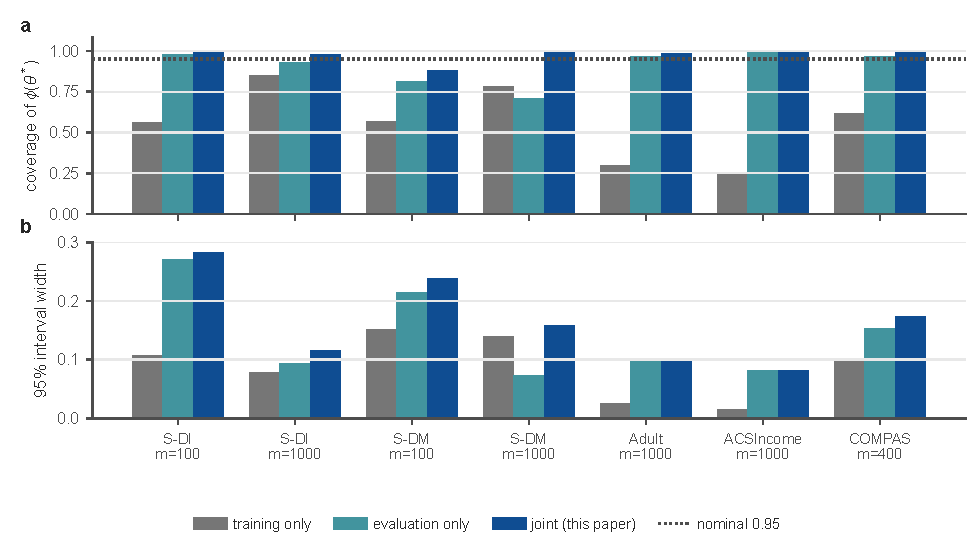
\includegraphics[width=\textwidth]{../results/figures/ablation_coverage.pdf}
\caption{Resampling both sources is the only variant that stays near nominal coverage in every
setting.  Source ablation under protocol (A) with nominal coverage $0.95$: intervals that resample
only the training trajectories, only the evaluation set, or both.  (a)~Coverage of the population
gap; the training-only interval undercovers in every setting, and the evaluation-only interval undercovers on the synthetic DM generator ($0.81$ at $m=100$), where the ignored training noise is large; the joint interval is at or near nominal level throughout.  (b)~The corresponding interval widths: valid inference costs little
beyond resampling the evaluation set, since the evaluation-only and joint intervals nearly coincide
on Adult and ACSIncome.}
\label{fig:ablation}
\end{figure}

\section{Discussion}
\label{sec:discussion}

Our results do not contradict the training-side theory of \citet{roy2026uq}; they delimit its scope.
Auditors should say which estimand an interval targets, and should not present an interval for the
held-out gap as an interval for the fairness of the deployed classifier.  Evaluation data should be
budgeted before training compute: in our experiments $m=1000$ labelled observations cannot certify a
gap to better than a few percentage points, whatever $T$ is.  Because the constraint set is itself a
random choice of audit design, a single constrained run should come with a constraint-set sensitivity
analysis.

\paragraph{Limitations.}
The theory inherits the asymptotic regime, strong convexity and linear/NTK classifier assumptions of
the baseline.  The joint bootstrap requires $\tbar_T$ to be close to $\theta^*$; unlike the evaluation
and constraint-set components, the optimisation bias is \emph{not} estimable from the same
single-stream bootstrap, and we only report its diagnostic (distance to a directly computed optimum)
and its effect (Table~\ref{tab:sensitivity}).  The constraint-set component assumes that resampling
$\Dp$ is meaningful, that is, that the audit tolerances and group definitions are exchangeable across
audits; when $\Dp$ is a fixed policy object rather than a random audit sample, this component should
be reported as a sensitivity analysis rather than folded into the interval.

Finally, the synthetic generator supplied by the baseline is close to degenerate: the protected
attribute is highly correlated with the label (correlation $0.83$).  Synthetic results are therefore a
mechanism check, not evidence about realistic fairness--accuracy trade-offs.  Extensions to multi-class criteria, intersectional group
collections and neural classifiers are left for future work.

\section{Conclusion}
\label{sec:conclusion}
Reported fairness gaps of online-trained classifiers carry three kinds of noise.  We showed that the
existing online bootstrap interval accounts only for training noise, derived how its coverage degrades
with the ratio of training to evaluation effort, and proposed a joint bootstrap that resamples the
training trajectories and the evaluation set, with a constraint-set layer for audits whose design is
random.  On three real audits, a variance budget attributes less than a tenth of the variability of a
reported gap to training noise; evaluation sampling dominates when the held-out set is small, and
constraint-set sampling can be the largest component of all.  Fairness audits should therefore budget
evaluation data and audit-design sensitivity before training compute, and should state which estimand
their interval targets.  Extending the analysis to sequential audit designs is left for future work.

\section*{Statements}

\paragraph{Data availability.} All datasets are public benchmarks (Adult, ACSIncome and COMPAS).
The processing scripts, data splits, training and bootstrap code, and raw per-repetition result
files are released under the MIT licence at \url{https://github.com/JoffinLu/FUQ}; a permanent
repository DOI (Zenodo) will be added when it is issued.  A complete reproduction report is
released with the code, and Appendix~\ref{app:repro} summarises the main deviations.

\paragraph{Code availability.} The complete code base (data preparation, estimators, online and
joint bootstrap, all experiment drivers, figure and table generation, and verification scripts)
is available at \url{https://github.com/JoffinLu/FUQ} under the MIT licence.

\paragraph{Funding.} This research received no specific grant from any funding agency.

\paragraph{Competing interests.} The authors declare no competing interests.

\paragraph{Ethics approval.} Not applicable. The study uses publicly available secondary datasets
(Adult, ACSIncome, COMPAS); no new human-subjects data were collected.

\paragraph{Consent to participate.} Not applicable.

\paragraph{Consent for publication.} Not applicable.

\paragraph{Authors' contributions.} C.L. conceived the study, developed the theory, implemented
the code, ran all experiments and wrote the manuscript. S.W. and X.L. validated the numerical
results, reviewed the code and revised the manuscript. All authors discussed the results, read and
approved the final manuscript.

\paragraph{Acknowledgements.} The authors thank the maintainers of the public data sets used in
this study.

\paragraph{Use of AI tools.} An AI-based assistant was used during the preparation of this
work: it helped implement and run the numerical experiments and draft and revise the text.  All
results reported here were re-checked against the released code and raw output files, and the
authors reviewed the manuscript in full and take responsibility for its content.

\appendix
\section{Proofs}
\label{app:proofs}

Throughout, $z_j=\mathbb{1}[z=j]$, $P_j=\Pr(z=j)$, $p_j=\Pr(h=1\mid z=j)$ and
$\hat P_j=m^{-1}\sum_{i\in\Dt}z_{i,j}$, $\bar\varphi_j=(\sum_{i\in\Dt}z_{i,j}\varphi_i)/\sum_{i\in\Dt}z_{i,j}$.

\subsection{Proof of Lemma~\ref{lem:eval}}
Write $A=\sum_{i}z_{i,1}\varphi_i$, $B=\sum_i z_{i,1}$, $C=\sum_i z_{i,0}\varphi_i$, $D=\sum_i z_{i,0}$.
Then $\dhat_m(\theta)=A/B-C/D$, $A/m\to P_1p_1$ and $B/m\to P_1$.  Direct computation gives
$\operatorname{Var}(A/m)=P_1p_1(1-P_1p_1)$, $\operatorname{Var}(B/m)=P_1(1-P_1)$ and
$\operatorname{Cov}(A/m,B/m)=P_1p_1(1-P_1)$, and analogously for $(C,D)$.  The delta method with
$J=(1/P_1,-p_1/P_1^2,-1/P_0,p_0/P_0^2)$ yields
\[
v^2(\theta)=\frac{p_1(1-p_1)}{P_1}+\frac{p_0(1-p_0)}{P_0},
\]
which also follows from the law of total variance by conditioning on the realised group memberships.
Independence of $\Dt$ from the training stream and $\Dp$ is part of Assumption~\ref{ass:base}.
For uniformity, the class of half-space indicators is a bounded VC class; on a fixed neighbourhood
of $\theta^*$ it is Donsker, so the empirical process is $O_p(m^{-1/2})$ uniformly in $\theta$.  On
shrinking neighbourhoods, $P(h_\theta(x)\neq h_{\theta^*}(x))\le L\|\theta-\theta^*\|$ for some
$L<\infty$ by the continuity of the feature densities at the boundary, and the same symmetrisation
argument (see \citealp{vdvwellner1996}, Ch.~2.3) gives a local oscillation of order
$o_p(m^{-1/2})+\|\theta-\theta^*\|$ uniformly over $\|\theta-\theta^*\|\le\delta_m$ for any
$\delta_m\to0$; this is what the linearisation step below uses.  The DM case only replaces the
indicator $h=1$ by $h=-1$ and yields a finite sum over the two label strata.

\subsection{Proof of Theorem~\ref{thm:limit}}
Add and subtract the evaluation estimand and split the error into three terms,
\begin{align*}
\sqrt T\big(\dhat_m(\tbar_T)-\Delta(\theta^*)\big)
&=\underbrace{\sqrt T\big(\Delta(\tbar_T)-\Delta(\theta^*)\big)}_{(i)}
+\underbrace{\sqrt T\big(\dhat_m(\theta^*)-\Delta(\theta^*)\big)}_{(ii)}\\
&\quad+\underbrace{\sqrt T\big[(\dhat_m-\Delta)(\tbar_T)-(\dhat_m-\Delta)(\theta^*)\big]}_{(iii)}.
\end{align*}
Term (i) converges to $\mathcal N(0,\sigma^2_\Delta)$ by Lemma~\ref{lem:train}.  For (iii), the map $\theta\mapsto(\Delta(\theta),P h_\theta)$ is differentiable on the neighbourhood of $\theta^*$ and the class of half-space indicators is Donsker, so the empirical process admits the linearisation $(\dhat_m-\Delta)(\theta)=(\dhat_m-\Delta)(\theta^*)+\nabla(\dhat_m-\Delta)(\theta^*)^\top(\theta-\theta^*)+o_p(m^{-1/2})$ uniformly for $\|\theta-\theta^*\|=O_p(T^{-1/2})$; the derivative is $O_p(m^{-1/2})$ and the displacement is $O_p(T^{-1/2})$ by Lemma~\ref{lem:train}, hence $(iii)=O_p(m^{-1/2})=o_p(1)$ as $m\to\infty$ in the regime $T/m\to\lambda$.  Term (ii) equals
$\sqrt{T/m}\,\sqrt m(\dhat_m(\theta^*)-\Delta(\theta^*))$, which by Lemma~\ref{lem:eval} converges to
$\mathcal N(0,\lambda v^2)$ and is independent of (i) by assumption.  Slutsky's lemma finishes the
proof.

\subsection{Proof of Corollary~\ref{cor:coverage}}
Let $\sigma_{\mathrm{tot}}^2=\sigma^2_\Delta+\lambda v^2$.  The interval of \citet{roy2026uq} has
half-width $z_{\alpha/2}\sigma_\Delta/\sqrt T$, hence
\[
\Pr\{\dhat_m(\tbar_T)\in I_T\}
=\Pr\Big\{\Big|\frac{\sqrt T(\dhat_m(\tbar_T)-\Delta(\theta^*))}{\sigma_{\mathrm{tot}}}\Big|
\le z_{\alpha/2}\frac{\sigma_\Delta}{\sigma_{\mathrm{tot}}}\Big\}+o(1)
=2\Phi\Big(z_{\alpha/2}\frac{\sigma_\Delta}{\sigma_{\mathrm{tot}}}\Big)-1 .
\]
The ratio $\sigma_\Delta/\sigma_{\mathrm{tot}}$ equals one if and only if $\lambda v^2=0$, so the
coverage equals $1-\alpha$ if and only if $m\gg Tv^2/\sigma^2_\Delta$.

\subsection{Proof of Remark~\ref{rem:protocol}}
With a fixed evaluation set, the interval error is
$\dhat_m(\tbar_T)-\Delta(\theta^*)=(\Delta(\tbar_T)-\Delta(\theta^*))+b$ with
$b=\dhat_m(\theta^*)-\Delta(\theta^*)$ fixed conditional on the evaluation set.  By
Lemma~\ref{lem:train},
\[
\Pr\Big\{\big|\sqrt T b+\sqrt T(\Delta(\tbar_T)-\Delta(\theta^*))\big|\le z_{\alpha/2}\sigma_\Delta\Big\}
=\Phi\big(z_{\alpha/2}-\sqrt T b/\sigma_\Delta\big)-\Phi\big(-z_{\alpha/2}-\sqrt T b/\sigma_\Delta\big)+o(1),
\]
which tends to zero for $|b|>0$; the simulations average this expression over the law of $b$, whose
standard deviation is $v/\sqrt m$.  This is the sense in which coverage statements about population
fairness require a fresh evaluation set.

\subsection{Proof of Theorem~\ref{thm:joint}}
Condition on the training data.  For a training multiplier trajectory,
$\sqrt T(\dhat_m(\bar\theta_T^{\,b})-\dhat_m(\tbar_T))=\sqrt T(\Delta(\bar\theta_T^{\,b})-\Delta(\tbar_T))+\sqrt T\big[(\dhat_m-\Delta)(\bar\theta_T^{\,b})-(\dhat_m-\Delta)(\tbar_T)\big]$;
by the online multiplier bootstrap theorem of \citet{roy2026uq} the first term has conditional law
converging to $\mathcal N(0,\sigma^2_\Delta)$, and the second is $o_p(1)$ by the same localisation
argument as in the proof of Theorem~\ref{thm:limit}, because both iterates lie within
$O_p(T^{-1/2})$ of each other.  The evaluation term
$\sqrt m(\dhat_{m,r}(\tbar_T)-\dhat_m(\tbar_T))$ is a standard empirical bootstrap of an i.i.d.\
sample: conditional on the data, the multinomial reweighting gives a conditional law converging to
$\mathcal N(0,v^2)$ by the same delta method as Lemma~\ref{lem:eval}.  The multiplier and evaluation
resamplings use independent randomness, so the two conditional laws are asymptotically independent;
after the rescaling of the main text this gives the law of
$\sqrt T(\dhat_m(\tbar_T)-\Delta(\theta^*))$.  For the third component, each resampled constraint set
yields $\theta^*_s$; when the resampled sets are i.i.d.\ from the audit design, the empirical
distribution over $s$ of $\dhat_m(\theta^*_s)-\dhat_m(\theta^*)$ converges to its sampling law as
$S\to\infty$, provided the constrained optima are estimated with $o_p(S^{-1/2})$ accuracy.  The
(modified) percentile interval is therefore asymptotically valid.  The folded interval for
$|\Delta(\theta^*)|$ has coverage at least that of the signed interval: if the signed interval $[l,u]$
contains $\Delta>0$ then $u\ge\Delta$ and hence $\max(|l|,|u|)\ge|\Delta|$; the case $\Delta<0$ is
symmetric, and when the signed interval contains both signs the folded interval is $[0,\max(|l|,|u|)]$
and covers $|\Delta|$ trivially.

\subsection{Derivation of the sample-size allocation}
Minimising $c_T T+c_m m$ subject to $z^2_{\alpha/2}(\sigma^2_\Delta/T+v^2/m)\le w^2$ has Lagrangian
$c_T T+c_m m+\mu(\sigma^2_\Delta/T+v^2/m-w^2/z^2_{\alpha/2})$.  The first-order conditions give
$T=\sigma_\Delta\sqrt{\mu/c_T}$ and $m=v\sqrt{\mu/c_m}$, hence
$m/T=(v/\sigma_\Delta)\sqrt{c_T/c_m}$.  Substituting into the constraint yields
$\sqrt\mu=z^2_{\alpha/2}(\sigma_\Delta\sqrt{c_T}+v\sqrt{c_m})/w^2$ and therefore
\[
T=\frac{z^2_{\alpha/2}}{w^2}\Big(\sigma^2_\Delta+\sigma_\Delta v\sqrt{c_m/c_T}\Big),
\qquad
m=\frac{z^2_{\alpha/2}}{w^2}\Big(v^2+\sigma_\Delta v\sqrt{c_T/c_m}\Big).
\]

\section{Reproduction details}
\label{app:repro}

The reproduction follows the published equations, with the deviations listed in
Table~\ref{tab:deviations}; the complete report, code and raw result files are released with this
paper.  No official implementation accompanies \citet{roy2026uq}, so the training procedures
(weighted dual averaging with slab projection for DI, penalised SGD for DM) and the online multiplier
bootstrap were re-implemented from the paper.  The most consequential deviations are the step sizes:
in the synthetic DI experiment the published step size $\eta_0=0.01$ leaves the averaged iterate far
from the constrained optimum even at $T=10^5$, so we used $\eta_0=0.1$; the synthetic DM generator
scales the loss by $R^2=500$ and required $\eta_0=0.03$ to avoid divergence.  On the real datasets we
regularised by $\kappa=0.1$ so that the constrained optimum is reached within the training horizon;
this choice is analysed in Table~\ref{tab:sensitivity}.  The released reproduction report records, for
every setting, the distance between the averaged iterate and the directly computed constrained
optimum, so that the size of the optimisation bias can be judged alongside the interval.

\begin{table}[t]
\centering
\footnotesize
\setlength{\tabcolsep}{4pt}
\caption{Deviations of the reproduction from the published settings (all other settings as in Table~1 of the original paper).  ``z-score'' refers to normalising real features before training.}
\label{tab:deviations}
\begin{tabular}{lccc}
\toprule
setting & baseline & ours & reason \\
\midrule
step size $\eta_0$ (synthetic DI) & 0.01 & 0.1 & convergence within $T=2\times10^4$ \\
step size $\eta_0$ (synthetic DM) & 0.01 & 0.03 & divergence under $R^2=500$ scaling \\
regularisation $\kappa$ (real) & $10^{-4}$ & 0.1 & reach constrained optimum \\
features (real) & raw & z-score & conditioning \\
repetitions (real) & 100/200 & 100--150 & compute budget \\
$\theta^*$ & trained & direct solve & evaluate estimand at constraint optimum \\
population $\phi(\theta^*)$ & held-out & full pool & estimand definition \\
\bottomrule
\end{tabular}
\end{table}

\bibliography{refs}
\end{document}
